%==============================================================================
% A Software-Only Smart Parking Management System
% IEEE single-column format (IEEEtran, journal/onecolumn option).
% Compile with pdflatex:
%     pdflatex smart_parking.tex   (run twice to resolve cross-references)
% No external .bib file is required: the bibliography is embedded below.
%==============================================================================
\documentclass[journal,onecolumn,11pt]{IEEEtran}
\IEEEoverridecommandlockouts

\usepackage[margin=1in]{geometry}
\usepackage{cite}
\usepackage{amsmath,amssymb,amsfonts}
\usepackage{algorithm}
\usepackage{algpseudocode}
\usepackage{graphicx}
\usepackage{textcomp}
\usepackage{xcolor}
\usepackage{url}
\usepackage{booktabs}
\usepackage{array}
\usepackage{tikz}
\usetikzlibrary{arrows.meta,positioning,calc,fit,backgrounds}

\def\BibTeX{{\rm B\kern-.05em{\sc i\kern-.025em b}\kern-.08em
    T\kern-.1667em\lower.7ex\hbox{E}\kern-.125emX}}

% Currency marker, avoiding a fontspec dependency for the rupee glyph.
\newcommand{\rs}{\text{INR}\,}
% Fixed-width paragraph column.
\newcolumntype{L}[1]{>{\raggedright\arraybackslash}p{#1}}

\begin{document}

\title{A Software-Only Smart Parking Management System with\\
Vision-Language Number Plate Verification, Demand-Responsive Pricing\\
and Lock-Serialized Capacity Control}

\author{%
\IEEEauthorblockN{Harshit Tiwari\IEEEauthorrefmark{1},
Ankit Vishwakarma\IEEEauthorrefmark{1},
Vishal Chaudhary\IEEEauthorrefmark{1},
Shailaja Kumari\IEEEauthorrefmark{1},
Pawan Kumar Mall\IEEEauthorrefmark{2}}
\\[2pt]
\IEEEauthorblockA{Department of Computer Science and Engineering\\
Madan Mohan Malaviya University of Technology, Gorakhpur, Uttar Pradesh, India\\
\IEEEauthorrefmark{1}B.Tech.\ (CSE) --- 2023021136, 20230221111, 2023021165, 2024022014\\
\IEEEauthorrefmark{2}Assistant Professor (Supervisor)}
}

\maketitle

%==============================================================================
\begin{abstract}
Urban parking is still largely managed with paper tickets, flat hourly tariffs
and no advance visibility of availability, which pushes queueing onto the road
outside the facility and leaves both overstay time and demand-side revenue
uncollected. Existing smart-parking research answers this with per-bay sensor
networks and dedicated automatic number plate recognition (ANPR) appliances, a
capital cost that small and mid-sized operators cannot justify. This paper
presents a \emph{software-only} smart parking management system in which a
commodity webcam and a browser replace both the bay sensor array and the ANPR
box: the gate image is uploaded to the application server and transcribed by a
general-purpose vision--language model, and the returned registration number is
verified against a pre-paid reservation before the barrier opens. We contribute
five mechanisms and their reference implementation. First, a tiered plate
matching procedure that composes character normalisation, an OCR-confusion
canonical form and a normalised Levenshtein similarity into a five-way gate
decision, so that an optical misread and a genuinely wrong vehicle produce
different outcomes rather than the single ``no match'' of an exact-string
comparison. Second, a bounded demand-responsive pricing function over exactly
four factors --- occupancy, peak window, location zone and day of week ---
whose combined multiplier is clamped and whose full breakdown is frozen onto
the booking, so that a later tariff change cannot alter a completed
transaction. Third, an overstay billing rule that measures excess dwell as the
difference between actual and expected exit, forgives a configurable grace
period, and charges the remainder per started hour at the rate the driver
actually paid. Fourth, a Redis distributed lock (\texttt{SET NX PX} with a
token-checked Lua release) that serialises the read--modify--write on facility
capacity, making the reservation, the reserved-to-occupied handover at entry
and the slot release at exit safe under concurrent requests and idempotent
under a double-firing camera. Fifth, an idempotent settlement path that
tolerates the two independent channels --- browser callback and gateway webhook
--- through which a capture notification arrives. The system is realised as a
modular monolith of eleven service-layer modules, 57 REST endpoints and eight
collections over Node.js, Express, MongoDB and Redis, with a React single-page
application serving driver, owner and administrator panels behind an Nginx
reverse proxy. A 39-case unit suite covering the pricing algebra, the billing
rule, plate matching and lock mutual exclusion passes in full, and every
external dependency degrades to a defined behaviour rather than failing the
request.
\end{abstract}

\begin{IEEEkeywords}
smart parking, automatic number plate recognition, vision--language models,
dynamic pricing, distributed locking, idempotence, modular monolith,
intelligent transportation systems.
\end{IEEEkeywords}

%==============================================================================
\section{Introduction}
\label{sec:intro}

\subsection{Motivation and Problem Statement}

Searching for a parking space is not a private inconvenience; it is a
measurable component of urban congestion. Shoup's field studies in dense
commercial districts attribute a substantial share of vehicle-kilometres on
central streets to drivers cruising for a curb space
\cite{shoup2006cruising,shoup2005highcost}, and argue that the underlying cause
is a price signal that does not move: when a space is underpriced relative to
demand, the queue rather than the tariff performs the rationing.

Off-street facilities exhibit five concrete deficiencies that a system design
can be held against. \emph{(i) No real-time visibility}: drivers cannot see
live availability before arriving, so facility selection is uninformed and a
wasted approach trip is common. \emph{(ii) Manual ticketing and gate queues}:
paper tickets and cash at the barrier put service time per vehicle in the tens
of seconds, and the resulting queue extends onto the carriageway, converting an
inside-the-facility problem into an on-the-road one. \emph{(iii) Static pricing}:
a flat hourly rate identical at 03:00 on a Tuesday and 19:00 on a Saturday
cannot respond to occupancy, time of day, location premium or day of week.
\emph{(iv) Unverified entry and overstay leakage}: without plate verification a
booking cannot be tied to a vehicle, a reservation is transferable, and
overstay goes unbilled because measuring it requires the exact entry and exit
instants of that specific vehicle. \emph{(v) Hardware-heavy deployments}: per-bay
sensors and dedicated ANPR appliances make installation and maintenance costly
for precisely the small operators that most need the efficiency.

The literature answers the first four convincingly but at the cost of the
fifth. The dominant architecture instruments each bay with an ultrasonic,
magnetometric or infrared sensor, aggregates readings over a wireless sensor
network, and publishes occupancy to a cloud service
\cite{khanna2016iot,lin2017survey,kotb2016review}. Vehicle identity, where
handled at all, is delegated to a dedicated ANPR appliance built from classical
plate localisation, segmentation and character classification stages
\cite{anagnostopoulos2008survey,du2013alpr}. Both halves impose a per-facility
capital and maintenance cost --- sensors fail individually and must be located
and replaced, ANPR units must be re-tuned per site --- that a fifty-bay
operator cannot amortise.

\subsection{Approach}

This paper takes the opposite position on hardware, beginning from two
observations.

First, the occupancy of a \emph{reservation-mediated} facility can be derived
exactly from the booking and session ledger, with no bay sensing at all,
provided the gate events that drive that ledger are trustworthy. A facility
that already operates a barrier has a natural choke point at which every
vehicle is observed; if each passage is recorded reliably, the difference
between capacity and recorded interior population \emph{is} the availability,
and per-bay sensing measures something the ledger already knows.

Second, a contemporary general-purpose vision--language model \cite{gemini2023}
performs plate transcription well enough, from a commodity webcam frame, to
replace a dedicated ANPR pipeline for gate verification. This is a weaker claim
than it appears, and the weakness is the point: gate verification is a
\emph{closed-set} problem. The system need not read an arbitrary plate
correctly in the abstract; it must decide whether the vehicle at the barrier
corresponds to one of a handful of bookings due at that facility in that hour.
Verification against a known candidate set tolerates transcription noise that
open-set recognition would not.

Removing the hardware, however, moves the difficulty rather than eliminating
it, and the technical substance of this paper lies in the four problems the
substitution creates. A general-purpose model returns a string and a
self-reported confidence, not a calibrated detection, and it will occasionally
confuse \texttt{O} with \texttt{0}. A booking ledger used as the source of
occupancy truth is correct only if concurrent updates to it are serialised ---
a property a physical sensor gets for free from physics. A gate camera fires
twice on a single arrival as a matter of routine, so every state transition it
drives must be idempotent. And a payment gateway delivers the same capture
notification through two independent channels, so settlement must be idempotent
as well. None of these arises in the sensor-based architecture.

\subsection{Contributions and Organisation}

We contribute: \emph{(1)} a tiered plate verification procedure (Section
\ref{sec:plate}) composing normalisation, an OCR-confusion canonical form and
normalised Levenshtein similarity \cite{levenshtein1966} into five
distinguishable gate outcomes, driven by a bounded candidate scan that makes
``wrong vehicle'' reachable as a decision at all; \emph{(2)} a bounded,
auditable four-factor pricing function (Section \ref{sec:pricing}) whose
breakdown is frozen onto the booking; \emph{(3)} an overstay billing rule
(Section \ref{sec:billing}) charging only the excess beyond the pre-paid
window, at the effective rate already quoted; \emph{(4)} a concurrency and
idempotence design (Section \ref{sec:concurrency}) placing every capacity
mutation inside a Redis distributed lock \cite{redislocks} with defined
degradation; and \emph{(5)} an idempotent payment settlement path (Section
\ref{sec:payments}). Section \ref{sec:architecture} describes the architecture
and data model, Section \ref{sec:implementation} the implementation, Section
\ref{sec:evaluation} the evaluation, and Sections
\ref{sec:limitations}--\ref{sec:conclusion} the limitations, applications and
future work.

%==============================================================================
\section{Related Work}
\label{sec:related}

\subsection{Sensor-Based Smart Parking}

Khanna and Anand \cite{khanna2016iot} present the canonical IoT parking
deployment: per-bay sensors report to a cloud backend, and a mobile application
displays and reserves free bays. Lin \emph{et al.} \cite{lin2017survey} survey
the field, separating the \emph{information} a system provides from the
\emph{mechanism} by which it is obtained, and observe that the sensing layer
dominates both deployment cost and failure rate. Kotb \emph{et al.}
\cite{kotb2016review} identify reservation--payment integration as the weakest
link in practice: many systems reserve but do not transact, leaving the
commercial half of the problem to a manual process at the barrier.

Our design departs from this line in the sensing layer only. We retain
reservation, guidance, live availability and --- unlike much of the surveyed
work --- integrated payment and settlement, but derive occupancy from a
transactional ledger whose transitions are driven by verified gate events.

\subsection{Automatic Number Plate Recognition}

Classical ANPR is a multi-stage pipeline, and the surveys by Anagnostopoulos
\emph{et al.} \cite{anagnostopoulos2008survey} and Du \emph{et al.}
\cite{du2013alpr} catalogue the accuracy of each stage and its sensitivity to
illumination, skew, plate condition and format variation. Two properties matter
here. Errors are overwhelmingly \emph{character-level}: a correctly localised
plate is usually read with one or two characters wrong rather than wholly
misread, and the confused pairs are systematic (\texttt{O}/\texttt{0},
\texttt{I}/\texttt{1}, \texttt{S}/\texttt{5}, \texttt{B}/\texttt{8}). And the
engineering cost of the illumination and skew sensitivity is per-site tuning
--- exactly the cost we are avoiding.

We instead treat plate reading as an instruction-following transcription task
for a multimodal model \cite{gemini2023}, prompted for strict JSON, pinned to
zero temperature and constrained by a response schema. The model is explicitly
instructed \emph{not} to correct towards a plausible registration format,
because a model that silently repairs its own misread destroys the evidence the
downstream fuzzy matcher needs, converting a recoverable character-level error
into an unrecoverable one or into a confident match against the wrong vehicle.
Its output is treated as untrusted text throughout. The systematic
character-level error mode documented in
\cite{anagnostopoulos2008survey,du2013alpr} is what makes the OCR-confusion
canonical form of Section \ref{sec:plate} effective rather than arbitrary.

\subsection{Pricing and Architectural Style}

Pierce and Shoup's evaluation of SFpark \cite{pierce2013getting} is the
reference result for demand-responsive parking pricing: block-level rates
adjusted periodically toward an occupancy target measurably moved occupancy
toward that target. The SFpark rule adjusts slowly, in scheduled steps, on
observed occupancy alone, which suits curb parking where the price must be
legible on a sign. Our function instead evaluates at quote time, because a
driver booking through an application can be shown the exact price for their
exact window before paying; combines four orthogonal factors multiplicatively;
and is bounded by an explicit clamp, reported to the client when it binds.

On structure, the microservices literature \cite{newman2021} recommends
decomposition along business capabilities while noting that distributed
transactions are the principal cost of premature decomposition; Fowler's
``monolith first'' argument \cite{fowler2015monolithfirst} states the
corresponding default. A booking, its payment, its parking session and its
final bill form a single transaction-shaped narrative over one consistency
boundary. We therefore adopt a \emph{modular monolith}: strict module
boundaries enforced at the service layer, inside one deployable process and one
database, with the seams placed where extraction would occur if scale later
demanded it. Table~\ref{tab:related} summarises the positioning; the comparison
is architectural rather than empirical, since the approaches differ in what
hardware they require and therefore in what they can observe.

\begin{table}[!t]
\caption{Positioning Against Prevailing Smart-Parking Architectures}
\label{tab:related}
\centering
\small
\begin{tabular}{@{}lccc@{}}
\toprule
\textbf{Property} & \textbf{Sensor IoT} \cite{khanna2016iot,lin2017survey}
  & \textbf{ANPR appliance} \cite{du2013alpr} & \textbf{This work} \\
\midrule
Per-bay hardware required        & yes      & no       & \textbf{no} \\
Dedicated gate hardware required & no       & yes      & \textbf{no} \\
Per-site sensor or model tuning  & per-bay calibration & yes & \textbf{no} \\
Bay-level occupancy              & yes      & no       & no \\
Facility-level occupancy         & yes      & partial  & \textbf{yes} \\
Booking bound to a vehicle       & no       & yes      & \textbf{yes} \\
Demand-responsive pricing        & rare     & no       & \textbf{yes} \\
Automatic overstay billing       & no       & partial  & \textbf{yes} \\
Integrated payment settlement    & rare \cite{kotb2016review} & no & \textbf{yes} \\
Gate refusal taxonomy            & n/a      & binary   & \textbf{five-way} \\
Detects a vehicle bypassing the gate & yes  & no       & no \\
\bottomrule
\end{tabular}
\end{table}

%==============================================================================
\section{System Architecture}
\label{sec:architecture}

\subsection{Requirements and Deployment}

The platform serves three roles with incompatible trust levels: a driver may
act only on their own bookings, an owner only on their own facilities, and an
administrator across the platform but without the ability to fabricate a
transaction. Drivers search by location, see a live price before paying,
reserve and pay, enter and exit through camera verification, and review history
and dues. Owners register facilities for approval, configure capacity, rates
and hours, tune the four pricing factors against a 24-hour simulation, monitor
reservations, sessions and the transaction ledger, read the recognition audit
trail, and operate the gate from a browser terminal. Administrators moderate
accounts, approve or deactivate facilities, set commission, and review
transactions, live activity and the fraud report.

Non-functionally the system must be correct under concurrency (availability
must never be oversubscribed), idempotent at both external boundaries, and
auditable in money (any amount charged must be reconstructible after the fact,
independent of the rules currently configured). Every gate request must
terminate in a decision a gate client can act on, and the loss of any optional
dependency must produce defined behaviour.

Four capabilities are excluded by specification and are therefore absent by
design rather than omission: \emph{booking cancellation}, \emph{refunds},
\emph{booking expiry}, and \emph{QR codes}. The first three remove an entire
class of reversal flows from the money path. The fourth is substantive: plate
verification replaces the QR code entirely, because a QR code identifies a
\emph{booking} and is transferable between vehicles, whereas a plate identifies
the \emph{vehicle} and is not.

Fig.~\ref{fig:arch} shows the deployment. A React single-page application and
the REST API are served from a single origin by an Nginx reverse proxy: static
assets directly, and \texttt{/api} proxied to the Node.js process. Collapsing
both onto one origin removes cross-origin request handling from the production
path entirely and exposes a single port.

\begin{figure}[!t]
\centering
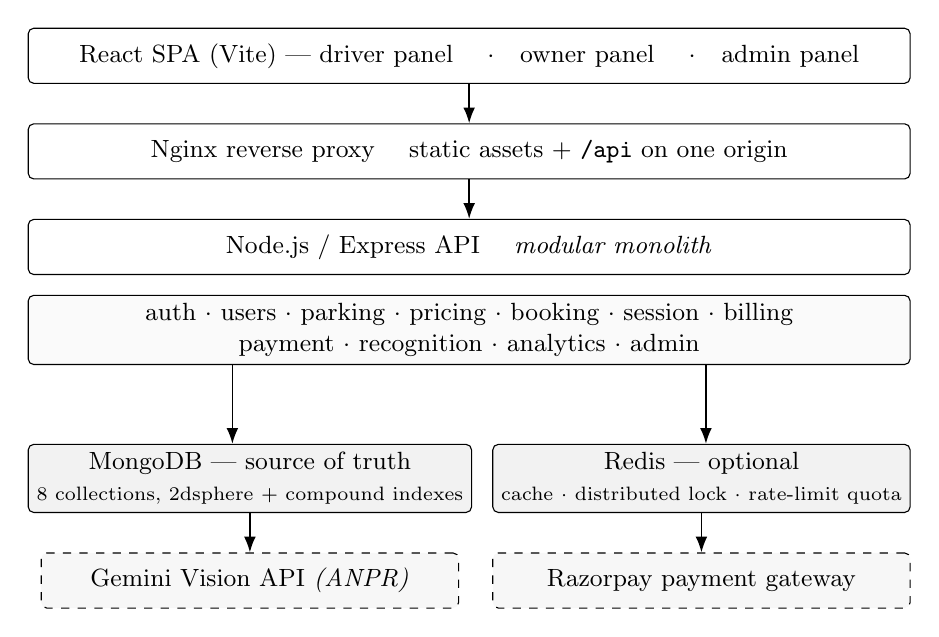
\begin{tikzpicture}[
  font=\small,
  box/.style={draw, rounded corners=2pt, minimum height=7mm, align=center,
              inner sep=3pt, fill=white},
  store/.style={box, fill=black!5},
  ext/.style={box, dashed, fill=black!3},
  arr/.style={-{Latex[length=2mm]}, semithick},
  node distance=5mm
]
\node[box, minimum width=112mm] (spa)
  {React SPA (Vite) --- driver panel \quad$\cdot$\quad owner panel \quad$\cdot$\quad admin panel};
\node[box, minimum width=112mm, below=of spa] (nginx)
  {Nginx reverse proxy \quad static assets $+$ \texttt{/api} on one origin};
\node[box, minimum width=112mm, below=of nginx] (api)
  {Node.js / Express API \quad \textit{modular monolith}};
\node[box, minimum width=112mm, below=2.5mm of api, fill=black!2] (mods)
  {auth $\cdot$ users $\cdot$ parking $\cdot$ pricing $\cdot$ booking $\cdot$ session $\cdot$ billing\\
   payment $\cdot$ recognition $\cdot$ analytics $\cdot$ admin};

\node[store, minimum width=53mm, below=10mm of mods.south west, anchor=north west]
  (mongo) {MongoDB --- source of truth\\\scriptsize 8 collections, 2dsphere $+$ compound indexes};
\node[store, minimum width=53mm, below=10mm of mods.south east, anchor=north east]
  (redis) {Redis --- optional\\\scriptsize cache $\cdot$ distributed lock $\cdot$ rate-limit quota};

\node[ext, minimum width=53mm, below=5mm of mongo] (gemini)
  {Gemini Vision API \textit{(ANPR)}};
\node[ext, minimum width=53mm, below=5mm of redis] (razor)
  {Razorpay payment gateway};

\draw[arr] (spa) -- (nginx);
\draw[arr] (nginx) -- (api);
\draw[arr] ($(mods.south west)+(26mm,0)$) -- ++(0,-10mm);
\draw[arr] ($(mods.south east)+(-26mm,0)$) -- ++(0,-10mm);
\draw[arr] (mongo) -- (gemini);
\draw[arr] (redis) -- (razor);
\end{tikzpicture}
\caption{Deployment architecture. The eleven modules are logical units inside
one process, not independently deployable services; they communicate only
through one another's service layers. Redis and both external providers are
optional at runtime and degrade to defined behaviour (Section
\ref{sec:degradation}).}
\label{fig:arch}
\end{figure}

\subsection{Module Decomposition}

Each module occupies its own directory with routes, controller, service and
validation files. Cross-module access is permitted only through an exported
service function, never by reaching into another module's models or routes,
which keeps the boundaries real despite the shared process.
Table~\ref{tab:modules} lists them with their dependencies, which is also the
extraction order should decomposition later become necessary.

One dependency is deliberately inverted: the \texttt{payment} module knows
nothing about bookings or sessions, and applying a captured payment to domain
state lives in a separate settlement unit that depends on both (Section
\ref{sec:payments}). Without this inversion the require graph would contain a
cycle --- booking creates a payment order, and a captured payment confirms a
booking --- and every settlement path would be harder to make idempotent.

\begin{table}[!t]
\caption{Module Responsibilities and Service-Layer Dependencies}
\label{tab:modules}
\centering
\small
\begin{tabular}{@{}lL{7.4cm}l@{}}
\toprule
\textbf{Module} & \textbf{Responsibility} & \textbf{Depends on} \\
\midrule
\texttt{auth}        & registration, login, refresh rotation, password change & --- \\
\texttt{users}       & driver dashboard aggregate, owner business profile & parking, booking \\
\texttt{parking}     & geospatial discovery, facility CRUD, ownership checks & pricing \\
\texttt{pricing}     & four-factor quote engine and owner rule editor & --- \\
\texttt{booking}     & reservation under the capacity lock, hold reclamation & pricing, payment \\
\texttt{session}     & parking session lifecycle, entry/exit transitions & billing, payment, parking \\
\texttt{billing}     & dwell time, overstay, final bill, receipt & pricing \\
\texttt{payment}     & order creation, signature verification, ledger & --- (gateway only) \\
\texttt{recognition} & gate decision engine and audit trail & booking, session, billing \\
\texttt{analytics}   & owner, per-facility and platform aggregates & --- (read-only) \\
\texttt{admin}       & account and facility moderation, commission, fraud & parking, payment \\
\bottomrule
\end{tabular}
\end{table}

\subsection{Data Model and the Capacity Invariant}
\label{sec:datamodel}

Eight MongoDB collections hold the domain (Table~\ref{tab:collections}). Two
modelling decisions recur. Every plate is stored twice --- as entered, and in a
normalised letters-and-digits-only form on which every comparison and index
lookup operates --- with normalisation performed in a pre-validate hook so the
two cannot drift. And recognition events store what the model returned but
never the image, so the audit trail can be retained indefinitely without
accumulating a corpus of photographs of identifiable vehicles.

\begin{table}[!t]
\caption{Collections and Their Principal Indexes}
\label{tab:collections}
\centering
\small
\begin{tabular}{@{}lL{6.9cm}L{5.1cm}@{}}
\toprule
\textbf{Collection} & \textbf{Holds} & \textbf{Principal index} \\
\midrule
\texttt{users} & accounts for all three roles, bcrypt hash, \texttt{tokenVersion}
  & \texttt{email} (unique) \\
\texttt{parkingOwners} & owner business profile, linked to a user
  & \texttt{user} \\
\texttt{parkingLots} & capacity, occupied and reserved triples, rates, hours,
  amenities, status, commission override, GeoJSON point
  & \texttt{location.geo} (2dsphere); \texttt{status} $+$ \texttt{city} \\
\texttt{pricingRules} & occupancy tiers, peak windows, zone factor, weekday
  multipliers, clamp limits
  & \texttt{parkingLot} \\
\texttt{bookings} & window, vehicle, normalised plate, frozen price snapshot,
  status, payment refs, fraud flags
  & \texttt{parkingLot} $+$ \texttt{plate} $+$ \texttt{status} $+$
    \texttt{expectedEntryTime} \\
\texttt{parkingSessions} & actual entry/exit, expected exit, status, final
  billing sub-document, entry and exit event refs
  & \texttt{parkingLot} $+$ \texttt{plate} $+$ \texttt{status} \\
\texttt{transactions} & ledger with purpose, amount, gateway identifiers and
  the settlement split frozen at capture
  & \texttt{parkingLot} $+$ \texttt{status} $+$ \texttt{createdAt} \\
\texttt{vehicleRecognitionEvents} & every gate capture: plate, confidence,
  latency, provider, result, allowed, match detail, fraud flag
  & \texttt{flaggedAsFraud} $+$ \texttt{createdAt} \\
\bottomrule
\end{tabular}
\end{table}

Capacity is the central piece of state. For a facility $\ell$ and vehicle class
$v \in \{\textit{two\_wheeler}, \textit{four\_wheeler}\}$ we store the physical
capacity $C_v$, the vehicles currently inside $O_v$, and the
paid-but-not-yet-arrived reservations $R_v$. The slots a new booking may take
and the occupancy ratio feeding the pricing engine are

\begin{equation}
  A_v \;=\; \max\bigl(0,\; C_v - O_v - R_v\bigr),
  \qquad\qquad
  \rho \;=\; \min\!\left(1,\;
    \frac{\sum_{v}\left(O_v + R_v\right)}{\sum_{v} C_v}\right).
  \label{eq:available}
\end{equation}

Counting a reservation as consumed capacity is what allows availability to be
correct in advance of arrival: a bay that has been paid for is not available to
anyone else, even though it is physically empty. The life of one slot is
therefore the three-step transfer shown in Fig.~\ref{fig:slot}, and each step
is a read--modify--write that must be serialised (Section
\ref{sec:concurrency}). The figure also gives the booking and session state
machines; note that a confirmed booking has no edge to a terminal state other
than through a completed session, which is the prohibition on cancellation and
expiry expressed structurally.

\begin{figure}[!t]
\centering
\begin{tikzpicture}[
  font=\small,
  st/.style={draw, rounded corners=3pt, minimum height=8mm, minimum width=24mm,
             align=center, inner sep=2pt, fill=white},
  cap/.style={st, fill=black!4},
  term/.style={st, fill=black!8},
  arr/.style={-{Latex[length=1.8mm]}, semithick},
]
% --- slot lifecycle ---
\node[font=\bfseries\small, anchor=west] at (-0.2,1.2) {(a) Slot lifecycle};
\node[cap] (free)  at (0,0)    {free\\\scriptsize in $A_v$};
\node[cap] (res)   at (3.9,0)  {reserved\\\scriptsize $R_v$};
\node[cap] (occ)   at (7.8,0)  {occupied\\\scriptsize $O_v$};
\node[cap] (free2) at (11.7,0) {free\\\scriptsize in $A_v$};
\draw[arr] (free) -- node[above,font=\scriptsize]{booking}
  node[below,font=\scriptsize]{$R_v\!+\!1$} (res);
\draw[arr] (res) -- node[above,font=\scriptsize]{verified entry}
  node[below,font=\scriptsize]{$R_v\!-\!1,\,O_v\!+\!1$} (occ);
\draw[arr] (occ) -- node[above,font=\scriptsize]{verified exit}
  node[below,font=\scriptsize]{$O_v\!-\!1$} (free2);
\draw[arr,dashed] (res.north) .. controls +(0,8mm) and +(0,8mm) ..
  node[above,font=\scriptsize]{unpaid hold reclaimed after 15\,min} (free.north);

% --- booking states ---
\node[font=\bfseries\small, anchor=west] at (-0.2,-2.0) {(b) Booking states};
\node[st] (bp) at (0,-3.2)   {pending\\payment};
\node[st] (bc) at (3.4,-3.2) {confirmed};
\node[st] (ba) at (6.8,-3.2) {active};
\node[term] (bd) at (10.2,-3.2) {completed};
\node[term] (bf) at (0,-5.0)  {payment\\failed};
\draw[arr] (bp) -- node[above,font=\scriptsize]{paid} (bc);
\draw[arr] (bc) -- node[above,font=\scriptsize]{entry} (ba);
\draw[arr] (ba) -- node[above,font=\scriptsize]{exit} (bd);
\draw[arr] (bp) -- node[right,font=\scriptsize]{failed / stale} (bf);

% --- session states ---
\node[font=\bfseries\small, anchor=west] at (-0.2,-6.2) {(c) Session states};
\node[st] (sa) at (0,-7.4)   {active};
\node[st] (sp) at (4.6,-7.4) {pending\\payment};
\node[term] (sc) at (9.2,-7.4) {closed};
\draw[arr] (sa) -- node[above,font=\scriptsize]{exit, $A_{\text{due}}>0$} (sp);
\draw[arr] (sp) -- node[above,font=\scriptsize]{settled} (sc);
\draw[arr] (sa.south) .. controls +(0,-9mm) and +(0,-9mm) ..
  node[below,font=\scriptsize]{exit, $A_{\text{due}}=0$} (sc.south);
\end{tikzpicture}
\caption{(a) Lifecycle of one parking slot: each transition is a
read--modify--write on the facility's capacity counters, executed inside the
distributed lock of Section \ref{sec:lock}. (b) and (c) the booking and session
state machines. The dashed edge is hold reclamation, which applies only to
bookings still awaiting payment and is not booking expiry.}
\label{fig:slot}
\end{figure}

Reservations are same-day only. A booking created but not yet paid holds its
slot for at most 15~minutes; the hold is reclaimed lazily, immediately before
the next capacity check on that facility, so an abandoned checkout can never
block a paying driver and no scheduler is required.

Driver-facing discovery is the hottest read path and is executed as a MongoDB
aggregation. When coordinates are supplied the pipeline opens with
\texttt{\$geoNear} against the \texttt{2dsphere} index so distance is computed
by the database and results arrive ordered by proximity; city and free-text
searches fall back to an indexed \texttt{find}. Search results are cached for
60\,s under a key derived from a hash of the query parameters, facility
availability for 30\,s, facility detail for 300\,s and analytics for 120\,s;
capacity mutations invalidate the first three, and pattern invalidation uses
\texttt{SCAN} with a bounded \texttt{COUNT} rather than \texttt{KEYS} so a
large keyspace is never blocked.

%==============================================================================
\section{Vision-Based Gate Verification}
\label{sec:recognition}

\subsection{Recognition Adapter}

The browser terminal captures a frame and posts it to the API, which sends the
image to the vision model's image-understanding endpoint \cite{googleaidocs}
with a fixed instruction prompt and a JSON response schema over four fields:
\texttt{plate} (nullable), \texttt{confidence}, \texttt{vehicleType} and
\texttt{notes}. The prompt states the task, forbids autocorrection, and defines
the null case explicitly: \textit{``Return ONLY the characters printed on the
plate, uppercase, with no spaces, dashes or state name. Do not guess or
auto-correct towards a plausible format. Transcribe exactly what is legible. If
the plate is unreadable, absent, or you are not confident, set plate to null.''}

Three generation parameters are pinned. Temperature is zero, because the task
is transcription rather than interpretation. The model's reasoning budget is
set to zero: plate transcription requires no deliberation, and on a thinking
model the reasoning tokens are drawn from the same output budget, so disabling
them both preserves the budget for the answer and approximately halves latency.
The output ceiling is 512 tokens against a payload of roughly thirty, so
exhaustion is structurally improbable --- and because an exhausted budget
yields an empty response indistinguishable from an unreadable plate, the finish
reason is logged separately to keep ``clean the camera'' distinguishable from
``raise the token budget''.

The response passes four checks before influencing a database lookup. It is
stripped of code fences and parsed as JSON, falling back to the first balanced
brace-delimited substring; an unparseable response is reported as an unreadable
plate, not a server error. The confidence is coerced and clamped to $[0,1]$,
with a non-finite value becoming zero, and the read is accepted only if
$c \geq \tau_{\text{conf}} = 0.55$. Finally the normalised string must match an
Indian registration shape --- two letters, one or two digits, up to three
letters, up to four digits --- or the BH series, with total length 6 to 11,
because a model can return a confidently formatted string that is not a plate
at all. An operator may also enter a plate manually, recorded with
\texttt{provider} $=$ \texttt{manual} so the audit trail distinguishes an
attendant's judgement from a machine read. The API key is held server-side and
sent as a request header rather than a query parameter, so it does not appear
in access logs; the frontend never contacts the model provider.

\subsection{Tiered Plate Matching}
\label{sec:plate}

Let $N(\cdot)$ denote normalisation --- uppercase, then delete every character
outside \texttt{[A-Z0-9]} --- and $K(\cdot)$ the canonical form obtained by
applying $N$ and then the OCR confusion map

\begin{equation}
  \Phi = \{\texttt{O},\texttt{Q},\texttt{D}\!\to\!\texttt{0};\;\;
           \texttt{I},\texttt{L}\!\to\!\texttt{1};\;\;
           \texttt{S}\!\to\!\texttt{5};\;\;
           \texttt{Z}\!\to\!\texttt{2};\;\;
           \texttt{B}\!\to\!\texttt{8};\;\;
           \texttt{G}\!\to\!\texttt{6}\}
  \label{eq:confusion}
\end{equation}

character-wise. The map is deliberately many-to-one and directed towards
digits, so it is idempotent and order-independent: $K(K(x)) = K(x)$, and two
strings differing only by confusable characters collapse to the same canonical
form regardless of which side the error occurred on. For a recognised plate $a$
and a booked plate $b$, with $d_L$ the Levenshtein distance
\cite{levenshtein1966},

\begin{equation}
  s(a,b) \;=\; 1 - \frac{d_L\bigl(K(a), K(b)\bigr)}
                       {\max\bigl(|K(a)|,\, |K(b)|\bigr)} \;\in\; [0,1].
  \label{eq:similarity}
\end{equation}

Normalising by the longer string bounds the score and makes it comparable
across plates of different length, which matters because the candidate scan
below ranks candidates by it. The comparison returns a \emph{kind} as well as a
score, and the gate decision is taken on the kind rather than the score alone
(Table~\ref{tab:tiers}).

\begin{table}[!t]
\caption{Plate Matching Tiers, with Worked Comparisons}
\label{tab:tiers}
\centering
\small
\begin{tabular}{@{}llcL{4.6cm}L{3.6cm}@{}}
\toprule
\textbf{Condition} & \textbf{Kind} & \textbf{$s$} & \textbf{Outcome}
  & \textbf{Example ($a$ vs.\ $b$)} \\
\midrule
$N(a) = N(b)$ & exact & $1.00$ & admit
  & \texttt{KA01AB1234} / \texttt{KA-01-AB-1234} \\
$N(a)\!\neq\!N(b)$, $K(a)\!=\!K(b)$ & ocr-equivalent & $0.98$ & admit
  & \texttt{KAO1ABI234} / \texttt{KA01AB1234} \\
$d_L \le 1$, $s \ge \tau_{\text{fuzzy}}$ & fuzzy & $\ge 0.85$
  & admit, flag for review
  & \texttt{KA01AB1235} / \texttt{KA01AB1234} \\
$s \ge \tau_{\text{susp}}$, above failing & mismatch & $\ge 0.60$
  & refuse, raise a fraud flag on the booking
  & near-miss on a booking due now \\
otherwise & --- & $< 0.60$ & refuse as an unbooked vehicle
  & \texttt{KA05CD7890} / \texttt{KA01AB1234} \\
\bottomrule
\end{tabular}
\end{table}

The \textsc{ocr-equivalent} tier covers a formatting artefact of the reader
rather than a different vehicle. The \textsc{fuzzy} tier requires \emph{both} a
unit edit distance and a similarity floor; the floor prevents a short plate, on
which one edit is a large fraction of the string, from being admitted on a
single-character difference. A fuzzy admission opens the barrier but is
recorded with a review flag, because the operational cost of stopping a
legitimate driver at a barrier exceeds the cost of reviewing the event
afterwards --- an asymmetry specific to this context that would not hold in,
say, access control for a secure area.

\subsection{The Candidate Scan}
\label{sec:candidates}

The distinction between \textsc{mismatch} and ``no booking'' cannot be drawn by
an exact-plate lookup, because a lookup on a misread plate returns nothing ---
exactly as it does for a car that never booked. Without an additional step the
\textsc{mismatch} branch is unreachable, and the system would wave an attempted
wrong-vehicle entry away as an unbooked car, losing precisely the fraud signal
the design exists to capture.

The entry path therefore performs a bounded candidate scan. Let $\mathcal{B}_t$
be the confirmed bookings at this facility admissible at instant $t$, that is
those whose booked interval $[t_{\text{in}}, t_{\text{out}}]$ satisfies

\begin{equation}
  t_{\text{in}} \leq t + \gamma_{\text{early}}
  \quad\text{and}\quad
  t_{\text{out}} \geq t - \gamma_{\text{late}},
  \qquad
  \gamma_{\text{early}} = 30\,\text{min},\;\;
  \gamma_{\text{late}} = 60\,\text{min}.
  \label{eq:window}
\end{equation}

The asymmetry is intentional: arriving early is a planning choice and can be
bounded tightly, whereas arriving late is usually caused by traffic and
deserves more tolerance. When the exact lookup fails, the engine computes
$\hat{b} = \arg\max_{b \in \mathcal{B}_t} s(a, b)$ and applies the tier rules to
that single best candidate.

The scan is bounded by construction: $\mathcal{B}_t$ is restricted to one
facility, a 90-minute window and a hard limit of 200 documents, and similarity
over plates of length $L \approx 10$ costs $O(L^2)$. The entry decision is
therefore $O(|\mathcal{B}_t| \cdot L^2)$ with $|\mathcal{B}_t| \leq 200$ --- a
few hundred microseconds, negligible beside the round trip to the vision model,
and incurred only when the exact lookup has already failed.

\subsection{The Gate Decisions}

Algorithm \ref{alg:entry} states the entry decision. The ordering of checks is
itself a design decision: the duplicate check precedes the booking lookup, so a
camera firing twice on one arrival is answered from the already-open session
rather than consuming a second booking; and the distinction between ``outside
the entry window'' and ``no booking'' is drawn only after the fraud-suspicion
branch, so a mismatched plate is never misreported as a timing problem.

\begin{algorithm}[!t]
\caption{Entry gate decision}
\label{alg:entry}
\small
\begin{algorithmic}[1]
\Require approved facility $\ell$, image or manual plate, instant $t$
\Ensure $(\textit{allowed}, \textit{result})$; every terminating path writes an audit event
\State $(a, c) \gets \Call{Recognise}{\text{image}}$
\If{$a = \varnothing$ \textbf{or} $c < \tau_{\text{conf}}$}
  \State \Return $(\textsc{false}, \textsc{unreadable})$
\EndIf
\State $\sigma \gets \Call{OpenSessionFor}{\ell, N(a)}$
\If{$\sigma \neq \varnothing$}
  \State \Return $(\textsc{true}, \textsc{duplicate})$
    \Comment{camera fired twice on one arrival; no state change}
\EndIf
\State $b \gets \Call{ExactAdmissibleBooking}{\ell, N(a), t}$;\quad
       $\hat{b} \gets \varnothing$
\If{$b = \varnothing$}
  \State $\hat{b} \gets \arg\max_{b' \in \mathcal{B}_t} s(a, b')$
    \Comment{bounded candidate scan, Section \ref{sec:candidates}}
  \If{$\hat{b} \neq \varnothing$ \textbf{and} $d_L \le 1$ \textbf{and}
       $s(a,\hat{b}) \ge \tau_{\text{fuzzy}}$}
    \State $b \gets \hat{b}$ \Comment{misread, but the same vehicle}
  \EndIf
\EndIf
\If{$b = \varnothing$}
  \If{$\hat{b} \neq \varnothing$ \textbf{and} $s(a,\hat{b}) \ge \tau_{\text{susp}}$}
    \State record fraud flag on $\hat{b}$;\quad
      \Return $(\textsc{false}, \textsc{plate\_mismatch})$
  \EndIf
  \If{$\Call{AnyOpenBooking}{\ell, N(a)} \neq \varnothing$}
    \State \Return $(\textsc{false}, \textsc{outside\_window})$
      \Comment{booked here, but not now}
  \EndIf
  \State \Return $(\textsc{false}, \textsc{no\_booking})$
\EndIf
\State $m \gets \Call{Compare}{a, b}$
\If{\textbf{not} $m.\textit{match}$ \textbf{or} $m.s < \tau_{\text{fuzzy}}$}
  \State record fraud flag on $b$;\quad
    \Return $(\textsc{false}, \textsc{plate\_mismatch})$
\EndIf
\State $\Call{OpenSession}{b, \ell, t}$
  \Comment{inside the capacity lock: $R_v \!-\! 1$, $O_v \!+\! 1$}
\State \Return $(\textsc{true}, \textsc{verified})$
\end{algorithmic}
\end{algorithm}

Exit is simpler in its matching --- the vehicle is matched against open sessions
rather than bookings --- but harder in its idempotence, because closing a
session moves money. The entire exit handler runs inside a per-vehicle lock
keyed on $(\ell, N(a))$. A plate with no open session is checked against
\emph{recently closed} sessions before being refused, so a second scan seconds
after a legitimate exit replays the original bill instead of raising a spurious
fraud flag. The final bill is computed, the session moves to
\textit{pending\_payment} or \textit{closed} according to whether anything is
owed, and the slot is released on the transition \emph{out of} the active state
rather than on every exit event --- so a repeated exit cannot decrement $O_v$
twice.

\subsection{Refusals as Outcomes}

A barrier requires a definite answer, and the refusal reasons demand different
responses from the attendant. The API therefore returns HTTP~200 with
\texttt{allowed:\ false} and a discriminated \texttt{result} field for all of
them (Table~\ref{tab:outcomes}). A 4\textit{xx} status would invite gate
clients to treat a legitimate refusal as a transport error and retry it, which
at a barrier means a queue.

\begin{table}[!t]
\caption{Gate Outcome Taxonomy}
\label{tab:outcomes}
\centering
\small
\begin{tabular}{@{}llL{9.4cm}@{}}
\toprule
\textbf{Result} & \textbf{Barrier} & \textbf{Meaning and operator response} \\
\midrule
\textsc{verified}        & open   & plate matched a booking (entry) or an open session (exit) \\
\textsc{duplicate}       & open   & camera fired twice; the original outcome is replayed \\
\textsc{unreadable}      & closed & plate could not be read; move the vehicle forward or enter it manually \\
\textsc{no\_booking}     & closed & no confirmed booking for this plate here; direct the driver to the booking flow \\
\textsc{outside\_window} & closed & booked here but outside the entry window; the response states by how many minutes \\
\textsc{plate\_mismatch} & closed & plate resembles a booking here but is not it; flagged as fraud, summon an attendant \\
\textsc{no\_session}     & closed & exit attempted with no open session; flagged \\
\bottomrule
\end{tabular}
\end{table}

Every capture is written to \texttt{vehicleRecognitionEvents} whether or not
the barrier opened --- a refusal is frequently the more interesting record ---
and the audit write is wrapped so its failure cannot stall the gate. The
administrator fraud report reads from this collection on the
\texttt{flaggedAsFraud} index.

%==============================================================================
\section{Demand-Responsive Pricing}
\label{sec:pricing}

\subsection{The Quote Function}

Let $r_{\text{base}}(v)$ be the facility's configured hourly rate for vehicle
class $v$. Four factors are evaluated for a booked window
$[t_{\text{in}}, t_{\text{out}}]$, and no others: the specification permits
exactly these, and the implementation exposes exactly these.

$m_{\text{occ}}$ is a step function of the live occupancy ratio $\rho$ from
\eqref{eq:available}, obtained by locating $\rho$ in the facility's ordered
tier table --- by default $1.0$ up to $50\%$, $1.15$ to $75\%$, $1.3$ to $90\%$
and $1.5$ thereafter: list price while there is plenty of space, rationing by
price as the facility fills. $m_{\text{peak}}$ is the maximum multiplier over
all configured peak windows overlapping the booked window on that weekday; a
booking touching any part of a window pays that premium, and overlapping
windows take the highest rather than the product, since two adjacent rush
windows would otherwise compound into a premium neither was configured to
express. Windows crossing midnight are handled by a wrap-around containment
test. $m_{\text{loc}}$ is a zone premium, either an explicit multiplier or a
preset ranging from $0.95$ (residential) through $1.0$ (standard), $1.15$
(commercial), $1.2$ (mall), $1.25$ (railway), $1.3$ (CBD) and $1.35$ (stadium)
to $1.4$ (airport). $m_{\text{dow}}$ is one multiplier per weekday, defaulting
to $1.15$ on Saturday, $1.10$ on Sunday, $1.05$ on Friday and $1.00$ otherwise.

The combined multiplier is their product, clamped to the facility's configured
band $[\mu_{\min}, \mu_{\max}]$ (default $[0.5, 2.5]$); billable hours charge
any started hour in full subject to a facility minimum $h_{\min}$; and the
effective rate and payable amount follow:

\begin{align}
  \mu &= \mathrm{clamp}\bigl(
    m_{\text{occ}} \cdot m_{\text{peak}} \cdot m_{\text{loc}} \cdot
    m_{\text{dow}},\; \mu_{\min},\, \mu_{\max}\bigr),
  \label{eq:mu}\\
  h &= \max\!\left(h_{\min},\;
    \left\lceil \frac{t_{\text{out}} - t_{\text{in}}}{60\,\text{min}}
    \right\rceil\right),
  \label{eq:hours}\\
  r_{\text{eff}} &= r_{\text{base}}(v)\cdot\mu,
  \qquad
  A = r_{\text{eff}} \cdot h .
  \label{eq:amount}
\end{align}

All monetary quantities are rounded to two decimal places at each step.
Table~\ref{tab:pricing} traces a representative quote end to end.

\begin{table}[!t]
\caption{Dynamic Pricing --- Worked Quote}
\label{tab:pricing}
\centering
\small
\begin{tabular}{@{}lL{7.8cm}r@{}}
\toprule
\textbf{Term} & \textbf{Source} & \textbf{Value} \\
\midrule
$r_{\text{base}}$   & configured four-wheeler rate                      & \rs 40.00 / h \\
$m_{\text{occ}}$    & $\rho = 0.82 \Rightarrow$ tier ``up to $0.90$''   & $1.30$ \\
$m_{\text{peak}}$   & booked window overlaps the evening rush (17:00--21:00) & $1.30$ \\
$m_{\text{loc}}$    & zone \textit{mall}                                & $1.20$ \\
$m_{\text{dow}}$    & Saturday                                          & $1.15$ \\
\midrule
raw product         & $1.30 \times 1.30 \times 1.20 \times 1.15$        & $2.33$ \\
$\mu$               & within $[0.5,\,2.5]$, clamp does not bind         & $2.33$ \\
$r_{\text{eff}}$    & $r_{\text{base}} \cdot \mu$                       & \rs 93.20 / h \\
$h$                 & 2\,h~10\,min, any started hour billed in full     & $3$ \\
\midrule
\textbf{$A$}        & $r_{\text{eff}} \cdot h$                          & \textbf{\rs 279.60} \\
\bottomrule
\end{tabular}
\end{table}

\subsection{Three Properties of the Design}

\textbf{Boundedness.} The clamp in \eqref{eq:mu} is not cosmetic. A driver
quoted a price on a screen before paying will not tolerate an unbounded surge,
and the multiplicative composition of four factors reaches
$1.5 \times 1.3 \times 1.4 \times 1.15 \approx 2.7$ under the default tables
alone. When the clamp binds, the response reports the pre-clamp value in a
\texttt{cappedFrom} field, so the bound is visible to the client and to the
owner's simulation rather than silently truncating.

\textbf{Immutability.} The complete price snapshot --- base rate, effective
rate, each of the four multipliers, the combined value and the line-item
breakdown --- is written onto the booking and never recomputed. A tariff change
made on Wednesday cannot alter, or even retrospectively re-explain, a booking
paid on Tuesday. This is what makes a charge reconstructible after the fact,
and what allows the overstay rule below to refer to ``the rate the driver
actually paid'' as a stored quantity rather than a recomputation.

\textbf{Server authority.} The quote endpoint exists so the driver sees the
price before paying, but the payable amount is re-derived on the server inside
the capacity lock at booking time (Algorithm \ref{alg:booking}, line 7). The
browser's quote is a preview with no authority over what is charged.

Owners configure all four tables through the facility panel. Because a
multiplicative rule over four factors is hard to reason about by inspection,
the editor renders a 24-hour simulation of the resulting tariff curve before
the rules are saved. Dynamic pricing may also be switched off per facility,
forcing all four multipliers to $1$ and reducing \eqref{eq:amount} to
$r_{\text{base}} \cdot h$.

%==============================================================================
\section{Session Billing and Overstay}
\label{sec:billing}

A booking is pre-paid, so at exit only the excess is newly owed. Let
$t_{\text{in}}^{a}$ and $t_{\text{out}}^{a}$ be the actual entry and exit
instants and $t_{\text{out}}^{e}$ the expected exit. Dwell time, overstay and
the chargeable remainder after a grace period $g$ are

\begin{equation}
  \Delta_{\text{park}} = t_{\text{out}}^{a} - t_{\text{in}}^{a},
  \qquad
  \Delta_{\text{over}} = \max\bigl(0,\;
    t_{\text{out}}^{a} - t_{\text{out}}^{e}\bigr),
  \qquad
  \Delta_{\text{chg}}  = \max\bigl(0,\; \Delta_{\text{over}} - g\bigr).
  \label{eq:overstay}
\end{equation}

The middle definition is worth stating explicitly because a natural alternative
is wrong. Overstay is the difference between actual and \emph{expected exit},
not between dwell time and booked duration: a driver who arrives 20 minutes
late for a two-hour booking and leaves at the booked exit time has parked for
1\,h\,40\,m and has not overstayed at all. Measuring against the expected exit
instant is what makes late arrival the driver's loss rather than the facility's
liability.

With penalty multiplier $\kappa$ (default $1.5$) the overstay charge, session
total and newly payable amount are

\begin{equation}
  A_{\text{over}} \;=\;
    \bigl(r_{\text{eff}} \cdot \kappa\bigr)\cdot
    \left\lceil \frac{\Delta_{\text{chg}}}{60\,\text{min}} \right\rceil,
  \qquad
  A_{\text{total}} \;=\; A + A_{\text{over}},
  \qquad
  A_{\text{due}} \;=\; A_{\text{over}}.
  \label{eq:overstaycharge}
\end{equation}

Three decisions here deserve comment. The penalty is applied to
$r_{\text{eff}}$ --- the rate the driver actually paid --- and not to
$r_{\text{base}}$, so a peak-hour premium already charged at booking is not
compounded a second time. Only $A_{\text{over}}$ is newly payable, because the
booked window was captured up front. And leaving early produces no refund: it
is recorded as a breakdown line for transparency, but the specification defines
no refund flow. Table~\ref{tab:overstay} works the scenarios the unit suite
asserts directly.

\begin{table}[!t]
\caption{Overstay Billing --- Scenarios
  (2\,h booking, $r_{\text{eff}} = \rs 50$/h, $A = \rs 100$, $g = 10$\,min,
   $\kappa = 1.5$)}
\label{tab:overstay}
\centering
\small
\begin{tabular}{@{}lrrrrrr@{}}
\toprule
\textbf{Scenario} & $\Delta_{\text{over}}$ & $\Delta_{\text{chg}}$
  & \textbf{started h} & $A_{\text{over}}$ & $A_{\text{total}}$
  & $A_{\text{due}}$ \\
\midrule
Left on time              & 0 min   & 0 min   & 0 & \rs 0.00   & \rs 100.00 & \rs 0.00 \\
Left 8 min late (grace)   & 8 min   & 0 min   & 0 & \rs 0.00   & \rs 100.00 & \rs 0.00 \\
Left 45 min late          & 45 min  & 35 min  & 1 & \rs 75.00  & \rs 175.00 & \rs 75.00 \\
Left 2\,h~20\,m late      & 140 min & 130 min & 3 & \rs 225.00 & \rs 325.00 & \rs 225.00 \\
Left 30 min early         & 0 min   & 0 min   & 0 & \rs 0.00   & \rs 100.00 & \rs 0.00 \\
\bottomrule
\end{tabular}
\end{table}

At exit the barrier opens even when the overstay is unpaid. The vehicle is
physically leaving; holding a slot for a car that has gone is strictly worse
for the facility than collecting the balance afterwards, and refusing exit to a
driver who cannot pay immediately converts a billing problem into a blocked
lane. The session therefore moves to \textit{pending\_payment} with
\texttt{amountDue} set, a payment order is created, the amount appears in the
driver's dues list, and the slot is released immediately. A receipt covering
dwell time, overstay, the rate applied and the line-item breakdown is returned
to the gate terminal and retained on the session.

%==============================================================================
\section{Concurrency, Idempotence and Degradation}
\label{sec:concurrency}

\subsection{The Race for the Last Slot}

The critical race is two drivers taking the last free bay at the same instant.
Both read $A_v = 1$ from \eqref{eq:available}, both conclude the booking is
admissible, and both decrement --- leaving $A_v = -1$ and one driver charged
for a bay that does not exist. Because the check and the write are separate
database operations, no single-document atomic update can prevent this: an
atomic decrement makes the \emph{write} indivisible but does nothing about the
window between reading the value and deciding to write. The two operations must
be made mutually exclusive.

\subsection{The Lock Protocol}
\label{sec:lock}

We use a Redis distributed lock keyed on the facility \cite{redislocks}.
Acquisition is \texttt{SET key token PX ttl NX}, which succeeds only if the key
is absent and sets an expiry in the same round trip. Release is a Lua script
evaluated server-side:

\begin{verbatim}
    if redis.call("GET", KEYS[1]) == ARGV[1] then
      return redis.call("DEL", KEYS[1])
    else
      return 0
    end
\end{verbatim}

The token check is the essential part. Without it, a holder whose critical
section overran the TTL would delete a lock Redis had since granted to someone
else, and two callers would be inside the critical section each believing they
held it. Evaluating the comparison and the delete as one Lua script makes that
check-and-delete atomic. The default TTL is 5\,s with up to 20 retries at
100\,ms; the entry handover uses 8\,s because it performs more work. Failure to
acquire after all retries returns HTTP~409 with a retry message rather than
silently proceeding --- the one outcome a capacity system must never produce is
a booking made without the check.

Algorithm \ref{alg:booking} gives the booking critical section. The essential
point is line 5: the facility document is \emph{re-read inside the lock},
because the copy fetched before acquisition may already be stale. A
re-validation using a pre-lock snapshot is not a check at all. Line 2 prevents
a subtler duplication --- one vehicle holding two overlapping reservations,
possibly at different facilities --- and includes unpaid holds, since otherwise
two pending checkouts for the same plate could both complete and produce
overlapping confirmed bookings.

\begin{algorithm}[!t]
\caption{Reservation under the capacity lock}
\label{alg:booking}
\small
\begin{algorithmic}[1]
\Require facility $\ell$, vehicle class $v$, window $[t_{\text{in}},t_{\text{out}}]$, driver $u$
\State validate the window: same day, not in the past, inside operating hours
\State reject if this plate already holds an overlapping booking anywhere on the platform
\State \textbf{acquire} $\textit{lock:lot:capacity:}\ell$
  \Comment{\texttt{SET NX PX}, up to 20 retries}
\State \Call{ReleaseStaleHolds}{$\ell$}
  \Comment{unpaid holds older than 15\,min: $R_v \!-\! 1$ each}
\State $\ell' \gets \Call{Reload}{\ell}$
  \Comment{re-read inside the lock}
\If{$A_v(\ell') \le 0$}
  \State \textbf{release}; \Return HTTP~409 \textit{no slots available}
\EndIf
\State $q \gets \Call{Quote}{\ell', v, t_{\text{in}}, t_{\text{out}}}$
  \Comment{server-authoritative, Eqs.~\eqref{eq:mu}--\eqref{eq:amount}}
\State create the booking with status \textit{pending\_payment} and the full snapshot $q$
\State $R_v \gets R_v + 1$
\State \textbf{release}; invalidate the availability, detail and search caches
\State \Return a payment order for $q.A$
\end{algorithmic}
\end{algorithm}

A booking is created before payment, not after. Holding the slot only after
payment means a driver can be charged for a slot taken by someone else while
they were on the payment page --- a refund problem in a system with no refund
flow. The cost is that an abandoned checkout sits on a slot, which is why
reclamation runs at line 4, inside the lock and immediately before the capacity
check. The same lock guards the $R_v \to O_v$ handover at entry and the $O_v$
decrement at exit, so the invariant \eqref{eq:available} holds across all three
transitions of Fig.~\ref{fig:slot}.

\subsection{Idempotence and Degradation}
\label{sec:degradation}

Two sources of duplicate events are treated as routine rather than
exceptional. \emph{Gate cameras} fire more than once per arrival: Algorithm
\ref{alg:entry} checks for an existing open session before searching for a
booking, and the exit path runs under a per-vehicle lock, replays the original
outcome for a recently closed session, and releases the slot only on the
transition out of the active state. \emph{Payment notifications} arrive through
both the browser callback and the gateway webhook for the same capture; Section
\ref{sec:payments} describes the settlement path that absorbs this.

Every external dependency has a defined failure behaviour rather than an
exception path (Table~\ref{tab:degradation}). The important nuance is the lock
fallback: an in-process lock still serialises requests within one Node
instance, which is correct for a single-instance deployment, but does not
provide the guarantee across a horizontally scaled fleet. It is therefore
logged at warning level on \emph{every} acquisition, so a Redis outage in a
multi-instance deployment is loud rather than subtly incorrect. A health
endpoint reports which dependencies are actually connected, so the degraded
mode is observable rather than inferred.

\begin{table}[!t]
\caption{Degradation Behaviour of External Dependencies}
\label{tab:degradation}
\centering
\small
\begin{tabular}{@{}lL{10.8cm}@{}}
\toprule
\textbf{Unavailable} & \textbf{Behaviour} \\
\midrule
Redis (cache)   & every read misses and falls through to MongoDB; correctness unaffected \\
Redis (lock)    & process-local lock; correct for a single instance, insufficient for a fleet, logged loudly on every acquisition \\
Redis (limiter) & per-instance in-memory counters instead of a shared quota \\
Vision model    & camera capture returns a configuration error; manual plate entry still exercises the entire gate flow end to end \\
Payment gateway & mock mode creates and signs orders locally, so booking $\to$ payment $\to$ entry $\to$ exit runs end to end; refuses to start under \texttt{NODE\_ENV=production} \\
\bottomrule
\end{tabular}
\end{table}

%==============================================================================
\section{Payment Orchestration and Settlement}
\label{sec:payments}

A payment order is created at booking, for the pre-paid amount $A$, and at
exit, for an unpaid overstay $A_{\text{due}}$. In both cases a
\texttt{transactions} document is written first, carrying the purpose, amount,
currency, gateway identifiers and --- once captured --- the settlement split.
An outstanding order for the same booking is reused rather than duplicated, so
a page refresh during checkout does not spawn a second order for the same slot.

Capture is verified three independent ways before any domain state changes. The
gateway signature over \texttt{orderId|paymentId} is recomputed with an
HMAC-SHA256 keyed on the API secret and compared in constant time, so a timing
side channel cannot be used to forge it byte by byte. The webhook signature is
computed over the \emph{raw} request body before any JSON parsing, because a
parse-then-reserialise round trip does not reproduce the exact bytes the
gateway signed. And the payment is fetched back from the gateway to confirm its
status and amount --- a signature proves the message came from the gateway, not
that the payment is still captured or that the amount is what the client
claimed.

Applying a captured transaction to domain state is isolated in a settlement
unit deliberately not part of the payment module. Architecturally this keeps
the payment module free of any dependency on bookings or sessions, so the
require graph stays acyclic; operationally, every branch is idempotent, because
a webhook and a browser callback routinely both arrive for the same payment in
an unspecified order. Settlement dispatches on purpose: a \textit{booking}
payment confirms the booking, an \textit{overstay} or \textit{final} payment
settles the session. A failed booking payment releases the capacity hold; a
failed overstay payment releases nothing, because an unpaid overstay is a debt
rather than a hold.

At capture the commission is computed from the facility's override percentage
when present and the platform default otherwise, and the resulting triple is
stored on the transaction:

\begin{equation}
  c = \frac{A \cdot p}{100},
  \qquad
  e = A - c,
  \label{eq:commission}
\end{equation}

where $p$ is the applicable percentage, $c$ the platform commission and $e$ the
owner earning. Storing the split at capture time rather than deriving it on
read means changing the platform rate later cannot rewrite what an owner has
already earned --- the same auditability principle that governs the price
snapshot.

Two paths bypass the gateway without bypassing the ledger. A fully discounted
booking has nothing to authorise and cannot raise a zero-value order, so it is
recorded as paid locally with a full transaction document, its settlement
breakdown and the reason no money moved, making it auditable rather than
invisible. And when no gateway credentials are configured the system runs in
mock mode, signing orders locally so the entire flow is exercisable in
development; mock mode refuses to start under \texttt{NODE\_ENV=production},
converting a dangerous misconfiguration into a startup failure.

%==============================================================================
\section{Security Design}
\label{sec:security}

Authentication uses short-lived JWT access tokens (15~min) with rotating
refresh tokens (7~days) \cite{rfc7519}, refreshed silently by the API client on
a 401. Each user document carries a \texttt{tokenVersion} embedded in issued
tokens and incremented on password change or deactivation; because the
middleware compares the token's version against the stored one, a single write
revokes every outstanding token for that user without a server-side session
store --- the standard objection to stateless tokens, answered with one
integer. Passwords are hashed with bcrypt \cite{provos1999bcrypt}.

Authorisation is layered. Role checks (\textit{user}, \textit{owner},
\textit{admin}) gate route families, and ownership checks additionally verify
that the requesting owner controls the facility being modified, performed in a
shared loader used by every owner-scoped route rather than repeated per
handler. Gate devices authenticate with a separate device key rather than a
user token, so a compromised gate terminal cannot act as a user and a leaked
user token cannot operate a barrier.

Input validation uses Zod schemas that \emph{replace} the validated request
part rather than merely inspecting it, so unknown keys are structurally unable
to reach a Mongoose model --- a mass-assignment defence that does not depend on
remembering to strip fields at each call site. Rate limits are Redis-backed so
the quota is shared across instances: 300 requests per 15~min globally, 20 per
15~min on authentication to blunt credential brute force, 30 per minute on
recognition because each call costs a paid model invocation, and 20 per minute
on payments. Helmet headers, an explicit CORS allowlist and compression are
applied at the application layer.

Two smaller decisions are worth recording. Login returns an identical failure
message for an unknown email and a wrong password, so the endpoint does not
disclose which accounts exist. And the process refuses to start in production if
the JWT secrets are still at their development defaults or the gateway is in
mock mode. Table~\ref{tab:security} summarises the controls.

\begin{table}[!t]
\caption{Security Controls and Enforcement Points}
\label{tab:security}
\centering
\small
\begin{tabular}{@{}L{6.8cm}L{7.4cm}@{}}
\toprule
\textbf{Control} & \textbf{Enforcement point} \\
\midrule
JWT access $+$ rotating refresh, silent refresh & token service; API client interceptor \\
\texttt{tokenVersion} mass revocation & user model; auth middleware \\
Role-based authorisation & auth middleware \\
Facility ownership checks & shared managed-facility loader \\
bcrypt password hashing & user model pre-save hook \\
Validation that replaces the request part & validation middleware \\
Redis-backed rate limiting & rate-limit middleware \\
Helmet, CORS allowlist, compression & application wiring \\
Constant-time gateway signature verification & gateway service \\
Raw-body webhook signature verification & application wiring; payment controller \\
Server-side model key, sent as a header & recognition service \\
Device-key authentication for gates & auth middleware \\
Plate-mismatch fraud flags & recognition service \\
Production refuses default secrets or mock payments & environment configuration \\
\bottomrule
\end{tabular}
\end{table}

%==============================================================================
\section{Implementation}
\label{sec:implementation}

The backend is Node.js~20 with Express~4 \cite{expressdocs}, Mongoose~8 over
MongoDB \cite{mongodocs}, and ioredis against Redis. The frontend is React~18
\cite{reactdocs} built with Vite, using an Axios client that holds the endpoint
map and the silent-refresh interceptor in one place. Payments settle through
the Razorpay gateway \cite{razorpaydocs}. Both tiers are containerised;
\texttt{docker-compose} brings up MongoDB, Redis, the API and an Nginx
container \cite{nginxdocs} serving the built SPA and proxying \texttt{/api}. A
seed script provisions demonstration data --- approved and pending facilities,
completed sessions including one with a billed overstay and one inside the
grace period, and one vehicle currently parked for exercising the exit gate.
Table~\ref{tab:scale} reports the scale, measured from the repository.

\begin{table}[!t]
\caption{Implementation Scale and REST API Surface (all routes under \texttt{/api/v1})}
\label{tab:scale}
\centering
\small
\begin{tabular}{@{}lr@{\qquad\qquad}lL{7.0cm}@{}}
\toprule
\textbf{Measure} & \textbf{Value} & \textbf{Module} & \textbf{Endpoints} \\
\midrule
Backend source files      & 71      & Auth & \texttt{POST /auth/register}, \texttt{/login}, \texttt{/refresh}, \texttt{/change-password}; \texttt{GET|PATCH /auth/me} \\
Backend lines of code     & 8{,}186 & Users & \texttt{GET /users/dashboard}; \texttt{GET|PATCH /users/owner-profile} \\
Logical modules           & 11      & Parking & \texttt{GET /parking/search}, \texttt{/:id}, \texttt{/:id/availability}, \texttt{/mine}, \texttt{/:id/manage}; \texttt{POST /parking}; \texttt{PATCH /parking/:id}; \texttt{POST /parking/:id/recount} \\
MongoDB collections       & 8       & Pricing & \texttt{POST /pricing/quote}; \texttt{GET|PUT /pricing/rules/:id}; \texttt{POST /pricing/rules/:id/simulate} \\
REST endpoints            & 57      & Bookings & \texttt{POST /bookings}; \texttt{GET /bookings/mine}, \texttt{/:id}, \texttt{/lot/:id} \\
Frontend components/pages & 41      & Sessions & \texttt{GET /sessions/mine}, \texttt{/lot/:id}, \texttt{/:id}, \texttt{/:id/preview-bill} \\
Frontend lines of code    & 10{,}500 & Payments & \texttt{GET /payments/config}, \texttt{/mine}, \texttt{/mine/dues}, \texttt{/lot/:id}; \texttt{POST /payments/booking-order}, \texttt{/session-order}, \texttt{/verify}, \texttt{/failed}, \texttt{/webhook} \\
Unit tests                & 39      & Recognition & \texttt{POST /recognition/entry}, \texttt{/exit}, \texttt{/preview}; \texttt{GET /recognition/status}, \texttt{/events/:id} \\
Unit test lines           & 473     & Analytics & \texttt{GET /analytics/owner}, \texttt{/lot/:id}, \texttt{/platform} \\
                          &         & Admin & \texttt{GET /admin/users}, \texttt{/users/:id}, \texttt{/lots}, \texttt{/transactions}, \texttt{/activity}, \texttt{/fraud}; \texttt{PATCH /admin/users/:id/status}; \texttt{POST /admin/lots/:id/review}; \texttt{PUT /admin/commission} \\
\bottomrule
\end{tabular}
\end{table}

Three role-specific interfaces are built on the same API, with the owner's gate
terminal the operationally distinctive one: it captures from a webcam, uploads
a photograph, or accepts a manually typed plate, and displays the barrier
decision, the matched booking, the session and, at exit, the full bill. A
read-only analytics module serves per-owner, per-facility and platform
dashboards over named time ranges, aggregating revenue and booking counts into
a gap-filled daily series and deriving average session duration and an
entry-hour distribution from the session collection.

%==============================================================================
\section{Evaluation}
\label{sec:evaluation}

\subsection{Correctness of the Monetary and Gate Logic}

We validate the components where an error either charges the wrong amount or
opens a barrier wrongly. The suite comprises 39 unit tests across four modules
and executes without MongoDB or Redis; the locking tests deliberately exercise
the no-Redis fallback path, since that is the path a single-instance deployment
actually takes. All 39 pass (Table~\ref{tab:tests}).

\begin{table}[!t]
\caption{Unit Test Results}
\label{tab:tests}
\centering
\small
\begin{tabular}{@{}lL{8.6cm}rl@{}}
\toprule
\textbf{Suite} & \textbf{Coverage} & \textbf{Cases} & \textbf{Result} \\
\midrule
pricing & base arithmetic (4); each of the four factors in isolation and the
          multiplier clamp (7); overstay quoting and the grace period (5)
        & 16 & pass \\
\addlinespace
plates  & normalisation (3); tiered comparison including OCR equivalence and
          fuzzy acceptance (6); format plausibility (2)
        & 11 & pass \\
\addlinespace
billing & final bill and overstay scenarios (6); duration formatting (1);
          receipt construction (1)
        &  8 & pass \\
\addlinespace
locking & mutual exclusion; last-slot contention; release on throw; value
          propagation
        &  4 & pass \\
\midrule
\textbf{Total} & & \textbf{39} & \textbf{39 pass} \\
\bottomrule
\end{tabular}
\end{table}

The \textbf{pricing} suite asserts the algebra of
\eqref{eq:mu}--\eqref{eq:amount} factor by factor: that a neutral configuration
charges exactly $r_{\text{base}} \cdot h$; that a started hour is billed in
full; that the two vehicle classes price independently; that a facility with no
rate for a class rejects the booking rather than defaulting; that each of the
four multipliers moves the price in isolation, including a peak window the
booking merely clips; that the clamp binds at $\mu_{\max}$; and that disabling
dynamic pricing reduces the function to the base rate. The \textbf{billing}
suite asserts \eqref{eq:overstay} directly --- overstay is
$t^{a}_{\text{out}} - t^{e}_{\text{out}}$ and not $\Delta_{\text{park}} - h$ ---
together with grace forgiveness, multi-hour overstay across started hours,
early exit recorded without refund, and that $A_{\text{due}}$ excludes the
pre-paid amount. The \textbf{plates} suite covers normalisation across
separators and case, the \texttt{O}$\leftrightarrow$\texttt{0} and
\texttt{I}$\leftrightarrow$\texttt{1} confusions collapsing under $K(\cdot)$,
single-character fuzzy acceptance, rejection of a genuinely different vehicle,
and the format predicate. The \textbf{locking} suite asserts that concurrent
callers are serialised, that exactly one of several contending callers can take
the last slot, that the lock is released when the critical section throws, and
that the return value propagates.

\subsection{Coverage of the Failure Modes This Design Introduces}

Section \ref{sec:intro} identified four correctness problems created by
removing the hardware. The OCR misread is addressed by the confusion-canonical
form and tiered matching, with 11 unit tests on the matcher but \emph{no
measured accuracy on real gate imagery}. Concurrent capacity updates are
addressed by the \texttt{SET NX PX} lock with token-checked release and the
re-read inside the lock, covered by four tests including last-slot contention.
The double-firing camera is addressed by the open-session check preceding the
booking lookup, the per-vehicle exit lock, the recently-closed replay and
release-on-transition; these are asserted structurally in Algorithm
\ref{alg:entry} and exercised by the seeded demonstration flow. Duplicate
payment notifications are addressed by the purpose-dispatched idempotent
settlement unit, whose separation from the payment module is enforced by the
acyclic require graph. Three of the four therefore have executable evidence;
the first does not, and that is the subject of Section \ref{sec:limitations}.

\subsection{Computational Cost and Threats to Validity}

Excluding the network round trip to the vision model, which dominates
end-to-end latency, the entry decision costs one indexed session lookup, one
indexed booking lookup, and in the worst case a bounded candidate scan of
$O(|\mathcal{B}_t| \cdot L^2)$ string comparisons with
$|\mathcal{B}_t| \leq 200$ and $L \approx 10$ --- incurred only when the exact
lookup fails. The exit decision costs one indexed session lookup plus the
constant-time billing arithmetic of
\eqref{eq:overstay}--\eqref{eq:overstaycharge}. On the recognition path itself,
disabling the model's reasoning budget is the single largest latency lever
available.

Three limits should be stated plainly. The unit suite establishes that the
monetary and matching \emph{logic} is correct given its inputs; it does not
establish that the vision model supplies correct inputs. The concurrency tests
exercise the in-process fallback lock rather than the Redis lock, so they
verify the serialisation contract and caller-visible behaviour but not the
Redis protocol under network partition. And no load test has been performed, so
the horizontal-scaling claim below is architectural rather than measured.

%==============================================================================
\section{Discussion and Limitations}
\label{sec:limitations}

\textbf{The ledger is not a sensor.} Occupancy is derived from verified gate
events, so a vehicle that physically bypasses the barrier is invisible and the
counters drift until an operator triggers a recount. Sensor-based designs
detect exactly this case. Our position is that a facility operating a barrier
already treats bypass as a physical-security problem, and that per-bay sensing
is a disproportionate answer to it --- but the limitation is real, and a
recount endpoint exists precisely because drift is possible. Relatedly, we
track $(C_v, O_v, R_v)$ per vehicle class per facility rather than the state of
individual bays, so in-facility guidance to a specific bay is out of scope:
adequate for a small or mid-sized facility, not for a multi-level structure
where finding the bay is itself the problem.

\textbf{Dependence on a hosted model.} Recognition requires connectivity to the
model provider, and its accuracy has not been measured on a controlled image
set in this work --- the most important gap in the evaluation. Behaviour under
an unavailable model is defined (manual entry), and the tiered matcher is
designed to absorb character-level misreads rather than assume they do not
occur, but neither substitutes for measured accuracy across illumination,
weather, plate condition and skew. Every gate capture is also a paid API call,
a recurring cost sensor-based designs do not have; the recognition rate limit
bounds it but does not eliminate it, and at high gate throughput the economics
may invert relative to a one-time appliance purchase.

\textbf{Uncalibrated thresholds.} $\tau_{\text{conf}} = 0.55$ gates on a
confidence the model reports about itself, which is not a calibrated
probability and may not be monotone in true accuracy. $\tau_{\text{fuzzy}} =
0.85$ and $\tau_{\text{susp}} = 0.6$ were chosen from the structure of Indian
plate formats and the properties of \eqref{eq:confusion}, not tuned against a
labelled corpus. The consequences of miscalibration are asymmetric: too low a
$\tau_{\text{fuzzy}}$ admits a wrong vehicle, while too high a value stops a
legitimate driver at the barrier.

\textbf{Scope boundaries.} Bookings are same-day by specification, excluding
multi-day airport parking --- a segment for which the overstay mechanism is
otherwise well suited. All timestamps are interpreted in a single configured
timezone, and the plate format predicate accepts Indian registration shapes
only; both are localisation boundaries rather than architectural ones, but
neither is currently parameterised per facility.

%==============================================================================
\section{Applications}
\label{sec:applications}

The software-only requirement --- a webcam, a browser and connectivity ---
makes the system deployable where a sensor retrofit would not be approved or
funded. \emph{Campus and institutional gates} can replace a paper pass with a
plate read at peak arrival times, where the bottleneck is service time at the
barrier rather than capacity inside. \emph{Airports and transit hubs} benefit
most from pre-booking combined with per-started-hour overstay billing, since
long-stay parking is where overstay leakage accumulates --- subject to lifting
the same-day constraint. \emph{Malls and multiplexes} are the natural fit for
zone-premium and day-of-week pricing following footfall through the day and
across the weekend; the 24-hour simulation exists largely for this audience.
\emph{Corporate campuses} can separate employee and visitor parking under one
ledger with per-facility commission and a full transaction record.
\emph{Hospitals and restricted zones} need precisely the property that
distinguishes this design from a QR code: entry verified against one specific
vehicle rather than one transferable token.

%==============================================================================
\section{Conclusion and Future Work}
\label{sec:conclusion}

We have presented a smart parking management system that eliminates per-bay
sensors and dedicated ANPR hardware by deriving occupancy from a reservation
ledger and delegating plate transcription to a general-purpose vision--language
model. The contributions are the mechanisms that make this substitution sound:
a tiered plate matcher with a bounded candidate scan that separates an optical
misread from a wrong vehicle, and thereby makes the mismatch case reachable at
all; a bounded, immutable, four-factor pricing function whose every charge
remains reconstructible after the rules change; an overstay rule that charges
only the excess, at the rate already paid, measured against the expected exit
rather than against dwell time; a distributed lock that serialises every
mutation of the capacity invariant while degrading to a stated weaker guarantee
when Redis is absent; and an idempotent settlement path tolerating duplicate
capture notifications from two independent channels. The implementation spans
11 modules, 57 endpoints and 8 collections over 18{,}686 lines of application
code, and its monetary and gate logic is covered by 39 unit tests, all passing.

Five directions follow. \emph{Measured recognition accuracy} is the most
pressing and the gap this paper is least able to close: a labelled corpus of
gate imagery stratified by illumination, weather, plate condition and skew
would allow $\tau_{\text{conf}}$, $\tau_{\text{fuzzy}}$ and
$\tau_{\text{susp}}$ to be calibrated against ground truth rather than chosen
from format structure, and would let the asymmetric costs of the two error
directions be priced explicitly. \emph{On-device edge ANPR} would run a local
model at the gate for offline operation with the hosted model as fallback,
removing both the connectivity dependency and the per-capture cost from the
critical path. \emph{Horizontal scaling} is already structurally available ---
the Redis lock makes multiple API instances behind Nginx upstreams safe --- and
remains to be load-tested, including the Redis protocol under partition rather
than only the in-process fallback. \emph{Selective extraction} of the
recognition and pricing modules, whose seams are already service-layer
boundaries and which have the fewest inbound dependencies in
Table~\ref{tab:modules}, is the natural first decomposition should independent
scaling become necessary. Finally, \emph{occupancy forecasting} from
accumulated session history would let the pricing function anticipate demand
rather than react to it, replacing the measured $\rho$ in \eqref{eq:available}
with a predicted value and moving the system from demand-responsive to
demand-anticipating pricing.

%==============================================================================
\section*{Acknowledgment}

The authors thank Dr.\ Pawan Kumar Mall of the Department of Computer Science
and Engineering, Madan Mohan Malaviya University of Technology, Gorakhpur, for
his supervision and guidance throughout this project.

%==============================================================================
\begin{thebibliography}{99}

\bibitem{shoup2006cruising}
D.~C. Shoup, ``Cruising for parking,'' \emph{Transport Policy}, vol.~13,
no.~6, pp. 479--486, 2006.

\bibitem{shoup2005highcost}
D.~C. Shoup, \emph{The High Cost of Free Parking}. Chicago, IL, USA: APA
Planners Press, 2005.

\bibitem{khanna2016iot}
A.~Khanna and R.~Anand, ``IoT based smart parking system,'' in \emph{Proc. Int.
Conf. Internet of Things and Applications (IOTA)}, Pune, India, 2016, pp.
266--270.

\bibitem{lin2017survey}
T.~Lin, H.~Rivano, and F.~Le~Mou\"{e}l, ``A survey of smart parking
solutions,'' \emph{IEEE Trans. Intell. Transp. Syst.}, vol.~18, no.~12, pp.
3229--3253, Dec. 2017.

\bibitem{kotb2016review}
A.~O. Kotb, Y.-C. Shen, and Y.~Huang, ``Smart parking guidance, monitoring and
reservation: A review,'' \emph{IEEE Intell. Transp. Syst. Mag.}, vol.~8, no.~2,
pp. 6--16, 2016.

\bibitem{anagnostopoulos2008survey}
C.~N.~E. Anagnostopoulos, I.~E. Anagnostopoulos, I.~D. Psoroulas, V.~Loumos,
and E.~Kayafas, ``License plate recognition from still images and video
sequences: A survey,'' \emph{IEEE Trans. Intell. Transp. Syst.}, vol.~9, no.~3,
pp. 377--391, Sep. 2008.

\bibitem{du2013alpr}
S.~Du, M.~Ibrahim, M.~Shehata, and W.~Badawy, ``Automatic license plate
recognition (ALPR): A state-of-the-art review,'' \emph{IEEE Trans. Circuits
Syst. Video Technol.}, vol.~23, no.~2, pp. 311--325, Feb. 2013.

\bibitem{gemini2023}
Gemini Team, Google, ``Gemini: A family of highly capable multimodal models,''
arXiv:2312.11805, 2023.

\bibitem{pierce2013getting}
G.~Pierce and D.~Shoup, ``Getting the prices right: An evaluation of pricing
parking by demand in San Francisco,'' \emph{J. Amer. Planning Assoc.}, vol.~79,
no.~1, pp. 67--81, 2013.

\bibitem{levenshtein1966}
V.~I. Levenshtein, ``Binary codes capable of correcting deletions, insertions
and reversals,'' \emph{Soviet Physics Doklady}, vol.~10, no.~8, pp. 707--710,
1966.

\bibitem{redislocks}
Redis Ltd., ``Distributed locks with Redis.'' [Online]. Available:
\url{https://redis.io/docs/latest/develop/use/patterns/distributed-locks/}

\bibitem{newman2021}
S.~Newman, \emph{Building Microservices: Designing Fine-Grained Systems},
2nd~ed. Sebastopol, CA, USA: O'Reilly Media, 2021.

\bibitem{fowler2015monolithfirst}
M.~Fowler, ``MonolithFirst,'' 2015. [Online]. Available:
\url{https://martinfowler.com/bliki/MonolithFirst.html}

\bibitem{rfc7519}
M.~Jones, J.~Bradley, and N.~Sakimura, ``JSON Web Token (JWT),'' RFC 7519,
IETF, May 2015.

\bibitem{provos1999bcrypt}
N.~Provos and D.~Mazi\`{e}res, ``A future-adaptable password scheme,'' in
\emph{Proc. USENIX Annu. Tech. Conf.}, Monterey, CA, USA, 1999, pp. 81--91.

\bibitem{googleaidocs}
Google, ``Gemini API: Image understanding.'' [Online]. Available:
\url{https://ai.google.dev/gemini-api/docs/image-understanding}

\bibitem{mongodocs}
MongoDB Inc., ``MongoDB manual --- geospatial queries.'' [Online]. Available:
\url{https://www.mongodb.com/docs/manual/geospatial-queries/}

\bibitem{expressdocs}
OpenJS Foundation, ``Express 4.x API reference.'' [Online]. Available:
\url{https://expressjs.com/en/4x/api.html}

\bibitem{reactdocs}
Meta Open Source, ``React documentation.'' [Online]. Available:
\url{https://react.dev/learn}

\bibitem{nginxdocs}
F5 NGINX, ``NGINX reverse proxy --- admin guide.'' [Online]. Available:
\url{https://docs.nginx.com/nginx/admin-guide/web-server/reverse-proxy/}

\bibitem{razorpaydocs}
Razorpay, ``Payment gateway documentation.'' [Online]. Available:
\url{https://razorpay.com/docs/}

\end{thebibliography}

\end{document}
